\documentclass[a4paper, 12pt]{article}

%Ukrainian language

\usepackage[T1,T2A]{fontenc}
\usepackage[utf8]{inputenc}
\usepackage[english,ukrainian]{babel}
\usepackage{indentfirst}

%Verbatim
\usepackage{fancyvrb}

%Math
\usepackage{amsmath,amsfonts,amssymb,amsthm,mathtools}

% Images
\usepackage{graphicx}
\usepackage{wrapfig}

%Vector graphics
\usepackage{tikz}
\usetikzlibrary{positioning}
\usetikzlibrary{patterns}

%Plots
\usepackage{pgfplots}
\pgfplotsset{compat=1.9}

%Title
\author{Демедюк Віталій Ігорович, студент 3 курсу, групи МІ}
\title{Науково-практичний звіт на тему\\
	   Побудова множини видимих та невидимих відрізків ребер 		       простого многокутника з точки}
\date{\today}

%Text color
\usepackage{xcolor}

%Multirow
\usepackage{multirow}

\usepackage{float}

\usepackage{bigstrut}
\usepackage{colortbl}

\usepackage[pdftex,
colorlinks,%
linkcolor=blue,citecolor=red,urlcolor=blue,
hyperindex,%
plainpages=false,%
bookmarksopen,%
bookmarksnumbered,%
unicode]{hyperref}

% For || ||
\usepackage{physics}

\begin{document}

\maketitle

\newpage
\tableofcontents

\newpage

\textbf{Анотація.} У роботі запропонований метод побудова множини видимих та невидимих відрізків ребер простого многокутника з точки. У цьому випадку задача була зведена до знаходження полігону видимості для відрізків, які не перетинаються, за винятком їх кінцевих точок.

\textbf{Abstract.} In the paper we proposes a method for constructing a set of visible and invisible segments of the edges of a simple polygon from a point. In this case, the problem was reduced to finding the polygon of visibility for segments that do not intersect, except for their endpoints.

\section{Вступ}

\textit{Постановка проблеми.} В роботі розглядається ідея розв'язку однієї з актуальних проблем обчислювальної геометрії -- знаходження множини видимих та невидимих відрізків ребер 		       простого многокутника з точки. Дана задача має як і наївні (неефективні) підходи до розв'язання, так і оптимізовані. Під час дослідження був запропонований досить ефективний метод, який добре себе показав на практиці.

\textit{Новизна та ідея.} Зведення задачі видимості ребер прямокутника з точки, до задачі знаходження полігону видимості для відрізків, які не перетинаються, за винятком їх кінцевих точок.

\textit{Мета статті.} Розробити алгоритм побудова множини видимих та невидимих відрізків ребер простого многокутника з точки 

\section{Основна частина}

\subsection{Постановка задачі}

Нехай задано простий многокутник $S$ з $N$ ребер на площині(в $E^d $ просторі). Також задано точку $A$. Потібно побудувати множину $U$ в яку входять усі фрагменти сторін многокутника $S$, до яких можна провести пряму з $A$ не перетнувши жодну з сторін прямокутника $S$.

\textbf{Означення 1.} Многокутника $P$ називається простим (або многокутником Жордана), якщо єдиними точками площини, що належать двом ребрам многокутника $P$, є вершини многокутника $P$. Такий многокутник має чітко визначені внутрішню і зовнішню частину.\cite{SimplePolygon}

\subsection{Зведення до задачі знаходження полігону видимості}

\textbf{Означення 2.} Формально ми можемо визначити задачу пошуку плаского полігона видимості наступним чином. Нехай $S$ -- множина перешкод (відрізків або многокутників) в $R^2$. Нехай $p$ -- точка в $R^2$, яка не міститься всередині перешкоди. Для точки $p$ многокутником видимості $V$ буде множина точок в $R$, таких, що для будь-якої точки $q$ з $V$, відрізок $pq$ не перетинає жодну перешкоду в $S$.\cite{VisibilityPolygon}

Таким чином, можемо звести нашу задачу до знаходження полігону видимості для нашої точки $A$ із однією перешкодою -- многокутником $S$. А множина $U$ буде складатися з усіх фрагментів сторін многокутника, які увійшли у полігон видимості.


\subsection{Алгоритм}

Для знаходження полігону видимості запропоновано безліч алгоритмів. Але нас цікавить вибір найефективнішого для розв'язання нашої задачі. Тому будемо розглядати алгоритми для побудови полігону видимості, де перешкодами у нас будуть відрізки, які не перетинаються, за винятком їх кінцевих точок.
Звернемо увагу, що будь-який алгоритм, який обчислює полігон видимості для точки серед відрізків, може бути використаний для обчислення многокутника видимості для всіх інших видів полігональних перешкод, оскільки будь-який полігон може бути розкладений на відрізки.

Одним із найефективніших алгоритмів на сьогоднішній час - техніка кутового замітання. Цей метод був запропонований у 1985\cite{AsanoTetsuo} та 1986\cite{SuriSubhash} рр.  Ефективна реалізація була опублікована в 2014 році.\cite{BungiuFrancisc}

Розглянемо одну з ефективних реалізацій - алгоритм Асано. Cпочатку нам потрібно відсортувати всі вершини вхідного многокутника за їхніми полярними кутами відносно точки запиту $q$. Сегменти, які перетинають промінь $L$, будемо зберігати у збалансованому двійковому дереві $T$ у порядку перетину з $L$. Під час змітання $T$ оновлюється, і нова вершина $V(q)$ генерується щоразу, коли найменший елемент (найближчий сегмент) до $q$) в $T$ змінюється.\cite{BungiuFrancisc}

\subsection{Часова складність}

Очевидно, що часова складнісь нашого алгоритму - $O(Nlog(N))$. Оскільки сортування вершин за полярним кутом швидше ніж за $O(Nlog(N))$ виконати ми не можемо. Процес замітання -- це прохід по відсортованому масиві з $N$ елементів. На кожному кроці проходу у нас може відбутися додавання елемента у збалансоване двійкове дерево, висота якого не перевищить $log(N)$. Тому складність нашого алгоритму -- $O(Nlog(N)) + O(N)O(log(N)) = O(Nlog(N))$.

\section{Практична частина}

У ході дослідження було розроблено програмну реалізацію алгоритму зазначеного вище мовою програмування \textit{C++}. Для графічно зображення результату було вибрано кросплатформенний інструментарій розробки користувацьких інтерфейсів \textit{Qt}. Програма надає користувачу два інтерфейси для введення вхідних даних: 1) ручний, через діалогове вікно; 2) завантаження даних з файлу. В правому нижньому куті програми потрібно вказати точку, з якої буде відбуватися побудова видимих відрізків. На основній частині користувацького інтерфейсу можемо побачити чорним кольором вказаний простий многокутник, а червоним кольором -- видимі відрізки.

\begin{figure}[H]
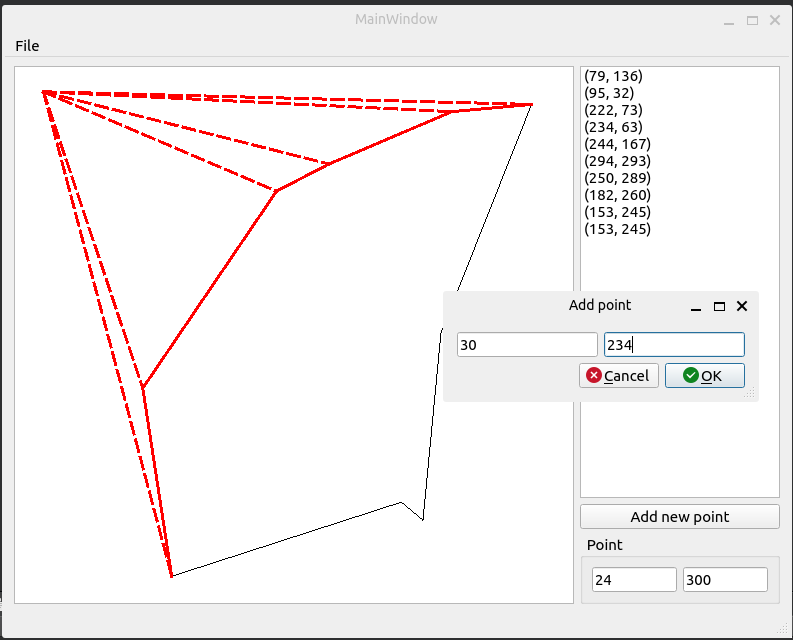
\includegraphics[scale=0.5]{img/UI.png}
\caption{Користувацький інтерфейс}
\end{figure}

\section{Висновки}

У роботі запропонований метод побудови множини видимих та невидимих відрізків ребер простого многокутника з точки. Звівши задачу до знаходження полігону видимості для відрізків, які не перетинаються, за винятком їх кінцевих точок, ми отримали ефективний алгоритм, який може використовуватись на практиці. Також даний метод можна використовувати, якщо нам потрібно розв'язати дану задачу одразу для декількох не перетинаючих простих многокутників. Це дуже добре, оскільки, як правило, на практиці нам потрібно мати справу одразу з декількома полігональними перешкодами. У ході дослідження також була розроблена ефективна навчальна програмна реалізація алгоритму, яку надалі можна розвинути до прикладного(комерційного) застосування.

\begin{thebibliography}{3}
\bibitem{SimplePolygon}
Weisstein, Eric W. Simple polygon Wolfram MathWorld.
\bibitem{VisibilityPolygon}
Visibility in simple polygons. Архів оригіналу за 3 травня 2017.
\bibitem{AsanoTetsuo}
Asano, Tetsuo (1985). An efficient algorithm for finding the visibility polygon for a polygonal region with holes. Institute of Electronics, Information, and Communication Engineers 68 (9). с. 557–559.
\bibitem{SuriSubhash}
Suri, Subhash; O'Rourke, Joseph (1986). Worst-case optimal algorithms for constructing visibility polygons with holes Symposium on Computational geometry. ACM. с. 14–23.
\bibitem{BungiuFrancisc}
Bungiu, Francisc; Hemmer, Michael; Hershberger, John; Huang, Kan; Kröller, Alexander (2014). «Efficient Computation of Visibility Polygons»
\end{thebibliography}


\end{document}